%1. Intro White-box, overview of analysis
%2. Explaining some analyzing strats that are out there
%3. VaRA, explain what vara does roughly (Regions)
%4. Vara TS Experiment explain
%5  TEF Report and how we evaluate them
%6. Using data to build multiple perf-influcence models


\colorlet{punct}{red!60!black}
\definecolor{background}{HTML}{EEEEEE}
\definecolor{delim}{RGB}{20,105,176}
\colorlet{numb}{magenta!60!black}
\lstdefinelanguage{json}{
    basicstyle=\normalfont\ttfamily,
    numbers=left,
    numberstyle=\scriptsize,
    stepnumber=1,
    numbersep=8pt,
    showstringspaces=false,
    breaklines=true,
    frame=lines,
    backgroundcolor=\color{background},
    literate=
     *{0}{{{\color{numb}0}}}{1}
      {1}{{{\color{numb}1}}}{1}
      {2}{{{\color{numb}2}}}{1}
      {3}{{{\color{numb}3}}}{1}
      {4}{{{\color{numb}4}}}{1}
      {5}{{{\color{numb}5}}}{1}
      {6}{{{\color{numb}6}}}{1}
      {7}{{{\color{numb}7}}}{1}
      {8}{{{\color{numb}8}}}{1}
      {9}{{{\color{numb}9}}}{1}
      {:}{{{\color{punct}{:}}}}{1}
      {,}{{{\color{punct}{,}}}}{1}
      {\{}{{{\color{delim}{\{}}}}{1}
      {\}}{{{\color{delim}{\}}}}}{1}
      {[}{{{\color{delim}{[}}}}{1}
      {]}{{{\color{delim}{]}}}}{1},
}


%************************************************
\section{White-box Analysis}\label{ch:Whitebox}
%************************************************
%Intro into White-Box with comparison to black-box
A black-box analysis is very useful for systems where we do not have access to the source code, but has drawbacks.
So, in the case where we have source code access, we should take advantage of this additional information to overcome some of the drawbacks.
Analyses that incorporate source code information are usually referred to as white-box analyses. 

In \autoref{ch:general-concepts}, introduce the general concepts behind white-box analysis and 
highlight current state-of-the-art strategies that employ white-box analysis in tho context of configurable software systems.
Subsequently, we present \textsc{VaRA}, a white-box analysis framework that focuses on the analysis of configurable software systems. 
In \autoref{ch:trace-event}, we explain how to build the {\perfInfluenceModel} using the white-box data.

\subsection{General Concept}\label{wb:general-concept}

While a black-box analysis measures the time we spend executing the system from start to finish, 
a white-box analysis archives a more fine grained view by using different strategies to determine how much time we spend in each feature, some of which
we further explain in \autoref{analyzing-strats}.

\mycomment{
To track features during the execution of the code, we declare variables that implement features as feature variables. 
During execution, these features taint parts of the code that are influenced by the value of the feature variable. 
A white-box analysis tracks the time for these tainted code parts.}

\begin{figure}[h]
    \centering
    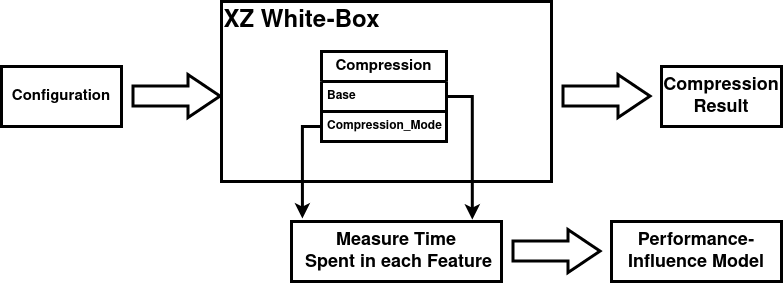
\includegraphics[scale=0.55]{gfx/whitebox_2.png}
    \caption{Process of using a white-box analysis to build a {\perfInfluenceModel} for \textit{XZ}.}
    \label{fig:WBxz}
\end{figure}

For example, let us take a look at a white-box analysis that analyses \textit{XZ} in \autoref{fig:WBxz} and compare this to how a black-box analysis would work.
Both analyses use different configurations containing the features and feature interaction we want to measure. 
The black-box analysis now would measure the time spent while the system is executed with the specific configuration.
However, the white-box analysis instead uses a strategy to measure the time spent in specific features. 
Afterwards, the black-box analysis would use a model, like multiple linear regression, to infer the time spent in each feature. 
However, the white-box analysis does not need this since we already measured the time spent in each feature, which we then use to build the {\perfInfluenceModel}.

\mycomment{
%Example of white-box pipeline
We now use a white-box analysis, to analyze the example system from \autoref{fig:xz}. 
In \autoref{fig:WBxz}, we have access to the source code of \textit{XZ}. 
Our first step is to manually analyze the code and find the feature variables that implement configurability inside the system. 
In this example, we found the feature \textit{Base} and \textit{compression\_mode}. 
During compression, we use our white-box analysis to measure the time spent by \textit{XZ} in the different features. 
This example measures the time spent in $Base$ and $Compression\_Mode$. 
After the system finished the process, we collected all the measurements generated by the white-box analysis, 
which we then used to build a {\perfInfluenceModel} for this configuration.
}

\subsection{VaRA}\label{VaRA}
%what is vara
To analyze the configurable software system we are interested in, we use \textsc{VaRA}, 
a framework that is built on \textsc{LLVM}.
In addition, we use the \textsc{VaRA Tool Suite}\footnote{Visited at 14.03.2022 \url{https://vara.readthedocs.io}}, which provides us with a framework that supports
us when analyzing configurable software systems with \textsc{VaRA}.
    
%Why vara
The purpose of \textsc{VaRA} is to provide various analyses for systems where the user only needs to focus on the high-level conceptual information of the 
system, while \textsc{VaRA} handles the low-level-details. 
Since \textsc{VaRA} is built on top of \textsc{LLVM}, it is able to analyze systems written in languages that can be compiled by \textsc{LLVM}, such as C, C++ or Rust~\cite{VaRA-Flo}.

We use \textsc{VaRA} as the core of our white-box analysis to measure the time spent inside each feature and feature interaction, from which we then build the {\perfInfluenceModel}.  

\subsubsection{Feature Region}
%What a feature region is
To analyze configurable systems, \textsc{VaRA} identifies code regions associated with a feature or feature interaction.
\textsc{VaRA} refers to such code regions that are influenced by feature decisions as \emph{feature region}. 
The first step for \textsc{VaRA} to be able to detect these regions is to find the feature variable that represents the features inside the code and mark them as
feature variables. 
A feature region is, therefore, a part of the code that is executed depending on the value of the feature variable. Whenever we detect a feature region,
we inject code into the system to measure the time spent in these regions. Therefore, after detection every feature region, the whole code is instrumentalized
by \textsc{VaRA} to measure the time spent in each feature region. 

\lstset{style=myStyle}
\begin{minipage}{\linewidth}
\begin{lstlisting}[caption={Feature region example. The feature variable is highlighted in orange and the feature region is highlighted in red.}
    ,language=C++,label={alg:Vara_feature_regions},escapechar=|, captionpos=b]
void encrypt() {
    bool |\textcolor{YellowOrange}{Encryption}|; //Feature Variable | \label{line:encryption_feature_variable} |
    assign_feature(Encryption); //Assigns true if Encryption is selected
    
    if(|\textcolor{YellowOrange}{Encryption}|) | \label{line:encryption} |
        |\textcolor{red}{foo();} |     | \label{line:foo} |
    else
        |\textcolor{red}{bar();} |      | \label{line:bar} |
}
\end{lstlisting}
\end{minipage}

%Feature region example
To illustrate this, we design a small function that encrypt files depending on if the encryption feature is selected.
In \autoref{alg:Vara_feature_regions}, we can see the structure of the $Encryption$ feature region. 
The feature variable in \autorefLine{line:encryption_feature_variable} represents whether $Encryption$ is selected or deselected and so, depending on $Encryption$, 
either the $then$ or $else$ branch is executed. 
Together, these two branches form an $Encryption$ feature region.

%Explain taint analysis
\subsubsection{Taint Analysis}
Before explaining \textsc{VaRA} feature region detection, we explain the concept behind a taint analysis since both approaches build upon this analysis.

The common usage of a taint analysis is in cybersecurity, where we trace the data flow of data that originates from an outsider or an untrusted source.
We track how the data is propagated through the system until it reaches a point where it is again accessible to the outside.
We call the access where the data is injected \emph{sources}, and the points where the data is exposed to the outside \emph{sinks}~\cite{TaintAnalysis}.

%Expains vra taint analysis
\textsc{VaRA} uses taint analysis, too however, in contrast to the common usage of a taint analysis, 
we are not interested in finding the sinks where data is leaked to the outside. However, instead, we are interested whenever instructions access our feature. 
For the taint analysis, \textsc{VaRA} uses feature variables as sources and instruction as sinks. Whenever an instruction accesses a feature variable, 
this instruction is tainted by that feature~\cite{VaRA-Janik}.

%Expain Dominator approach
\paragraph{Dominator Approach}
We call the second approach the \emph{Dominator Approach}, in here, \textsc{VaRA} uses domination relationships to identify feature regions.

To do this, \textsc{VaRA} works with basic blocks of the control flow graph, whereas a basic block is an instruction sequence that contains an entry label, 
which is the entry point for the code, and a terminator at the end, which determine the control flow of the block. 
An example of a terminator is an if condition that uses a feature variable.

To discover these domination relationships, \textsc{VaRA} checks out which basic block dominates other basic blocks with dependent terminator instructions. 
A basic block $BB_1$ dominates a different basic block $BB_2$ when the terminator of $BB_1$ decides if $BB_2$ is executed. 
Now instructions in $BB_2$ would depend on the terminator instruction of $BB_1$. 
The feature for the feature region of $BB_2$ is the feature that corresponds to the feature variable used by the terminator of $BB_1$~\cite{VaRA-Tom}.

\subsubsection{Locating feature variables}
\textsc{VaRA} is not able to automatically detect which variables represent features. 
Therefore, we need to provide \textsc{VaRA} with information about the location of feature variables. One way to do this is by giving \textsc{VaRA}
a feature model as a \textsc{XML} file containing every feature's location inside the code.

\begin{minipage}{\linewidth}
\begin{lstlisting}[caption={Feature model of \autoref{alg:Vara_feature_regions} in XML. The start of a feature variable is highlighted in red and the
    end is highlighted in green.},
    language=XML,label={alg:Encrypton_feature_model_xml},escapechar=|, captionpos=b]
<locations>                               | \label{XML:location} |
    <sourceRange category="necessary">    | \label{XML:source_range} |
        <path>src/my_encryption.c</path>      | \label{XML:file_path} |
        |\textcolor{red}{<start>}|                             | \label{XML:start_variable} |
            <line>2</line>
            <column>10</column>
        |\textcolor{red}{</start>}| 
        |\textcolor{Green}{<end>}|                                 | \label{XML:end_variable} |
            <line>2</line>
            <column>19</column>
        |\textcolor{Green}{</end>}|
        </sourceRange>
</locations>
\end{lstlisting}
\end{minipage}

%XML Lplained
In \autoref{alg:Encrypton_feature_model_xml} we show how we encode the \emph{Encryption} feature from \autoref{alg:Vara_feature_regions} as a
feature variable. To do so we specify different tags inside the \emph{XML}.
The location tag contains, at least one \emph{<sourceRange>} tag, in which we specify the feature variable that is associated with the feature, 
however a location can contain multiple source ranges, whereas the feature is implemented by multiple feature variables.
Each \emph{<sourceRange>} tag contains a \emph{<path>} tag that specifies the location of the file containing the feature variable.
After specifying the path, we need even further to specify the location of the feature variable inside the file. 
For this, we see in \autorefLine{XML:start_variable} the \emph{<start>} tag and in \autorefLine{XML:end_variable} the \emph{<end>} tag, 
inside both, we specify the \emph{<line>} and \emph{<column>} for where the feature variable starts end ends. 

%Explained on example
For \autoref{alg:Vara_feature_regions}, we would specify that the feature variable
$Encryption$ is in \autorefLine{line:encryption_feature_variable} and begins in \emph{column 10} and ends in \emph{column 19}.

\subsubsection{VaRA Tool Suite}
%Explain Vara Tool Suite
We use \textsc{VaRA} in combination with the \textsc{VaRA Tool Suite}, a framework written in python that assists us 
when analyzing configurable software systems using \textsc{VaRA} by specifying an \emph{experiment} to analyze a particular \emph{project}. 
The result our analysis produces is written into a \emph{report}. We emphasize that both experiments and projects are independent, 
allowing us to use different experiments to analyze a project in different ways.
To start the analysis, we use the command-line tool \emph{vara-run}, which specifies which experiments we want to run for which project.

\subsection{Trace Event Format}\label{ch:trace-event}
%Introduce TEF report and purpose
When we use \textsc{VaRA} the code of the configurable software system gets instrumented to measure the time spent inside each feature region.
All these measurements are collected in a trace event format (TEF)
\footnote{Visited at 15.03.2022 \\ \url{https://docs.google.com/document/d/1CvAClvFfyA5R-PhYUmn5OOQtYMH4h6I0nSsKchNAySU}} report,
which we use to calculate the overall time spent in each feature and feature interaction to build the {\perfInfluenceModel}.

Every time we enter or leave a feature region, a trace event is triggered that contains the following information:\\

\begin{minipage}{\linewidth}
\begin{lstlisting}[caption={Example of a feature region trace entry in the TEF file},captionpos=b,language=json,firstnumber=1,label={event}]
"name": "Base",
"cat": "Feature",
"ph": "B",
"ts": 0,
"pid": 726119,
"tid": 726119,
"args": {
    "ID": 0
}
\end{lstlisting}
\end{minipage}
%Expain all the keys meaning
In \autoref{event}, we see how a trace event is structured. Each trace event contains a $name$ that refers to the names of the features that affect this
region, $ph$ represents the event type, while $B$ signals the beginning and $E$ the end of an event.
All events contain a timestamp $ts$ that refers to the time in milliseconds when the event began or ended.
$Args$ contain an $ID$ that refers to each event, so the event that initiates the beginning $E$ of a region has the same $ID$ as the event that signals when
we leave the region with $E$.

\begin{figure}[h]
    \centering
    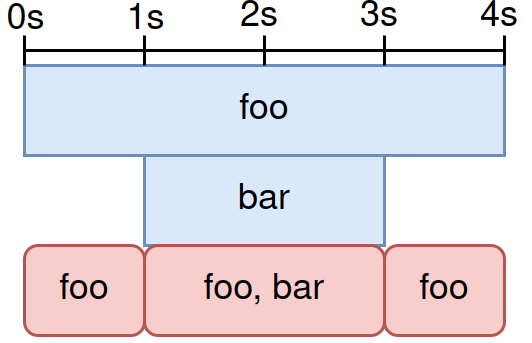
\includegraphics[scale=0.25]{gfx/trace_event_grafic.png}
    \caption{Example of two features interaction. Features are highlighted in blue and all the current active features are highlighted in red.}
    \label{fig:trace_event_grafic}
\end{figure}

%explain feature interaction time spent
When a trace event for a feature region begins before a trace event for a different feature ends, we say these features interact. 
As an example in \autoref{fig:trace_event_grafic}, we have two features, \emph{foo} and \emph{bar}, where the trace event of \emph{foo} starts at \emph{0} and ends at \emph{4} seconds 
and the trace event of \emph{bar} starts at \emph{1} and ends at \emph{3} seconds. We spent \emph{2} seconds in feature \emph{foo}, 
from \emph{0 to 1} and \emph{3 to 4}, 
but since we did not leave the feature region \emph{foo} before entering \emph{bar} we have an interaction between these features. 
Therefore, we spent \emph{2} seconds inside the feature interaction \emph{(foo, bar)} instead of the feature \emph{bar}.

%Expain order of interaction is irrelevant
Since we are only interested in which features interact, we ignore the order in which the interaction happens, which means the previous
interaction of \emph{(foo, bar)} is the same as \emph{(bar, foo)}. This also makes sense in the context of {\perfInfluenceModel} since we defined
the interaction of features as a product, where the time spent in that feature interaction is added if all features of that interaction are selected,
in this case, $2 \cdot c(foo) \cdot c(bar)$. Since the product is commutative, we also ignore the order in which the features interact inside the \perfInfluenceModel.

%Expain nesting
When we have nested trace events of the same feature, we do not add a feature interaction between the same features, 
due to the reason that inside the {\perfInfluenceModel} the feature interaction $2 \cdot c(foo) \cdot c(foo)$ is the same as $2 \cdot c(foo)$.

After the system finishes its execution, we have to transform the TEF report into a {\perfInfluenceModel} by aggregating all events. 
To do so, we sum up all the time spent in each region and attribute this time to the feature that influenced that region. 

We calculate the time spent on each feature as follows:

\mycomment{\begin{algorithm}
    \caption{Time spent in each feature \label{alg:performanceExample}}
    \textbf{Input:} feature_trace_event, a list containing features and
    \begin{algorithmic}[1]
    \text
    \State $\textit{features} \gets \textit{list}$\label{alg:code_insertion}

    \end{algorithmic}
    \end{algorithm}
}

\begin{align}
    \text{time(feature)} &= \textit{ }\textit{ }\textit{ } \sum_{\text{event} \in \text{feature}} \left( \sum_{(ts_E, ts_B) \in \text{event}} ts_E - ts_B \right) \label{math:time} \\ \nonumber \\
    \text{feature\_coefficients} &= \sum_{\text{feature} \in \text{TEF Report}}\text{time(feature)} \label{math:coefficients}
\end{align}

In \autoref{math:time}, we calculate the time spent for the given feature. 
For this equation, we define that a \textit{feature} as a list of \textit{events}, 
whereas each event is a pair of trace events representing when the feature region is entered and when it is left. 
To calculate the time spent in the region, we compute $ts_E - ts_B$.

\autoref{math:coefficients} is a sequence of the total time spent in each feature or feature interaction we measured in the \textit{TEF Report}. 
Now that we obtained all the coefficients that represent the influence of each feature and feature interaction, we use them to build the \perfInfluenceModel.
By that, we build up a {\perfInfluenceModel} from feature specific white-box performance measurements.